\documentclass{ximera}

%\usepackage{todonotes}

\newcommand{\todo}{}

\usepackage{esint} % for \oiint
\ifxake%%https://math.meta.stackexchange.com/questions/9973/how-do-you-render-a-closed-surface-double-integral
\renewcommand{\oiint}{{\large\bigcirc}\kern-1.56em\iint}
\fi


\graphicspath{
  {./}
  {ximeraTutorial/}
  {basicPhilosophy/}
  {functionsOfSeveralVariables/}
  {normalVectors/}
  {lagrangeMultipliers/}
  {vectorFields/}
  {greensTheorem/}
  {shapeOfThingsToCome/}
  {dotProducts/}
  {partialDerivativesAndTheGradientVector/}
  {../productAndQuotientRules/exercises/}
  {../normalVectors/exercisesParametricPlots/}
  {../continuityOfFunctionsOfSeveralVariables/exercises/}
  {../partialDerivativesAndTheGradientVector/exercises/}
  {../directionalDerivativeAndChainRule/exercises/}
  {../commonCoordinates/exercisesCylindricalCoordinates/}
  {../commonCoordinates/exercisesSphericalCoordinates/}
  {../greensTheorem/exercisesCurlAndLineIntegrals/}
  {../greensTheorem/exercisesDivergenceAndLineIntegrals/}
  {../shapeOfThingsToCome/exercisesDivergenceTheorem/}
  {../greensTheorem/}
  {../shapeOfThingsToCome/}
  {../separableDifferentialEquations/exercises/}
  {vectorFields/}
}

\newcommand{\mooculus}{\textsf{\textbf{MOOC}\textnormal{\textsf{ULUS}}}}

\usepackage{tkz-euclide}
\usepackage{tikz}
\usepackage{tikz-cd}
\usetikzlibrary{arrows}
\tikzset{>=stealth,commutative diagrams/.cd,
  arrow style=tikz,diagrams={>=stealth}} %% cool arrow head
\tikzset{shorten <>/.style={ shorten >=#1, shorten <=#1 } } %% allows shorter vectors

\usetikzlibrary{backgrounds} %% for boxes around graphs
\usetikzlibrary{shapes,positioning}  %% Clouds and stars
\usetikzlibrary{matrix} %% for matrix
\usepgfplotslibrary{polar} %% for polar plots
\usepgfplotslibrary{fillbetween} %% to shade area between curves in TikZ
%\usetkzobj{all}
\usepackage[makeroom]{cancel} %% for strike outs
%\usepackage{mathtools} %% for pretty underbrace % Breaks Ximera
%\usepackage{multicol}
\usepackage{pgffor} %% required for integral for loops



%% http://tex.stackexchange.com/questions/66490/drawing-a-tikz-arc-specifying-the-center
%% Draws beach ball
\tikzset{pics/carc/.style args={#1:#2:#3}{code={\draw[pic actions] (#1:#3) arc(#1:#2:#3);}}}



\usepackage{array}
\setlength{\extrarowheight}{+.1cm}
\newdimen\digitwidth
\settowidth\digitwidth{9}
\def\divrule#1#2{
\noalign{\moveright#1\digitwidth
\vbox{\hrule width#2\digitwidth}}}




% \newcommand{\RR}{\mathbb R}
% \newcommand{\R}{\mathbb R}
% \newcommand{\N}{\mathbb N}
% \newcommand{\Z}{\mathbb Z}

\newcommand{\sagemath}{\textsf{SageMath}}


%\renewcommand{\d}{\,d\!}
%\renewcommand{\d}{\mathop{}\!d}
%\newcommand{\dd}[2][]{\frac{\d #1}{\d #2}}
%\newcommand{\pp}[2][]{\frac{\partial #1}{\partial #2}}
% \renewcommand{\l}{\ell}
%\newcommand{\ddx}{\frac{d}{\d x}}

% \newcommand{\zeroOverZero}{\ensuremath{\boldsymbol{\tfrac{0}{0}}}}
%\newcommand{\inftyOverInfty}{\ensuremath{\boldsymbol{\tfrac{\infty}{\infty}}}}
%\newcommand{\zeroOverInfty}{\ensuremath{\boldsymbol{\tfrac{0}{\infty}}}}
%\newcommand{\zeroTimesInfty}{\ensuremath{\small\boldsymbol{0\cdot \infty}}}
%\newcommand{\inftyMinusInfty}{\ensuremath{\small\boldsymbol{\infty - \infty}}}
%\newcommand{\oneToInfty}{\ensuremath{\boldsymbol{1^\infty}}}
%\newcommand{\zeroToZero}{\ensuremath{\boldsymbol{0^0}}}
%\newcommand{\inftyToZero}{\ensuremath{\boldsymbol{\infty^0}}}



% \newcommand{\numOverZero}{\ensuremath{\boldsymbol{\tfrac{\#}{0}}}}
% \newcommand{\dfn}{\textbf}
% \newcommand{\unit}{\,\mathrm}
% \newcommand{\unit}{\mathop{}\!\mathrm}
% \newcommand{\eval}[1]{\bigg[ #1 \bigg]}
% \newcommand{\seq}[1]{\left( #1 \right)}
% \renewcommand{\epsilon}{\varepsilon}
% \renewcommand{\phi}{\varphi}


% \renewcommand{\iff}{\Leftrightarrow}

% \DeclareMathOperator{\arccot}{arccot}
% \DeclareMathOperator{\arcsec}{arcsec}
% \DeclareMathOperator{\arccsc}{arccsc}
% \DeclareMathOperator{\si}{Si}
% \DeclareMathOperator{\scal}{scal}
% \DeclareMathOperator{\sign}{sign}


%% \newcommand{\tightoverset}[2]{% for arrow vec
%%   \mathop{#2}\limits^{\vbox to -.5ex{\kern-0.75ex\hbox{$#1$}\vss}}}
% \newcommand{\arrowvec}[1]{{\overset{\rightharpoonup}{#1}}}
% \renewcommand{\vec}[1]{\arrowvec{\mathbf{#1}}}
% \renewcommand{\vec}[1]{{\overset{\boldsymbol{\rightharpoonup}}{\mathbf{#1}}}}

% \newcommand{\point}[1]{\left(#1\right)} %this allows \vector{ to be changed to \vector{ with a quick find and replace
% \newcommand{\pt}[1]{\mathbf{#1}} %this allows \vec{ to be changed to \vec{ with a quick find and replace
% \newcommand{\Lim}[2]{\lim_{\point{#1} \to \point{#2}}} %Bart, I changed this to point since I want to use it.  It runs through both of the exercise and exerciseE files in limits section, which is why it was in each document to start with.

% \DeclareMathOperator{\proj}{\mathbf{proj}}
% \newcommand{\veci}{{\boldsymbol{\hat{\imath}}}}
% \newcommand{\vecj}{{\boldsymbol{\hat{\jmath}}}}
% \newcommand{\veck}{{\boldsymbol{\hat{k}}}}
% \newcommand{\vecl}{\vec{\boldsymbol{\l}}}
% \newcommand{\uvec}[1]{\mathbf{\hat{#1}}}
% \newcommand{\utan}{\mathbf{\hat{t}}}
% \newcommand{\unormal}{\mathbf{\hat{n}}}
% \newcommand{\ubinormal}{\mathbf{\hat{b}}}

% \newcommand{\dotp}{\bullet}
% \newcommand{\cross}{\boldsymbol\times}
% \newcommand{\grad}{\boldsymbol\nabla}
% \newcommand{\divergence}{\grad\dotp}
% \newcommand{\curl}{\grad\cross}
%\DeclareMathOperator{\divergence}{divergence}
%\DeclareMathOperator{\curl}[1]{\grad\cross #1}
% \newcommand{\lto}{\mathop{\longrightarrow\,}\limits}

% \renewcommand{\bar}{\overline}

\colorlet{textColor}{black}
\colorlet{background}{white}
\colorlet{penColor}{blue!50!black} % Color of a curve in a plot
\colorlet{penColor2}{red!50!black}% Color of a curve in a plot
\colorlet{penColor3}{red!50!blue} % Color of a curve in a plot
\colorlet{penColor4}{green!50!black} % Color of a curve in a plot
\colorlet{penColor5}{orange!80!black} % Color of a curve in a plot
\colorlet{penColor6}{yellow!70!black} % Color of a curve in a plot
\colorlet{fill1}{penColor!20} % Color of fill in a plot
\colorlet{fill2}{penColor2!20} % Color of fill in a plot
\colorlet{fillp}{fill1} % Color of positive area
\colorlet{filln}{penColor2!20} % Color of negative area
\colorlet{fill3}{penColor3!20} % Fill
\colorlet{fill4}{penColor4!20} % Fill
\colorlet{fill5}{penColor5!20} % Fill
\colorlet{gridColor}{gray!50} % Color of grid in a plot

\newcommand{\surfaceColor}{violet}
\newcommand{\surfaceColorTwo}{redyellow}
\newcommand{\sliceColor}{greenyellow}




\pgfmathdeclarefunction{gauss}{2}{% gives gaussian
  \pgfmathparse{1/(#2*sqrt(2*pi))*exp(-((x-#1)^2)/(2*#2^2))}%
}


%%%%%%%%%%%%%
%% Vectors
%%%%%%%%%%%%%

%% Simple horiz vectors
\renewcommand{\vector}[1]{\left\langle #1\right\rangle}


%% %% Complex Horiz Vectors with angle brackets
%% \makeatletter
%% \renewcommand{\vector}[2][ , ]{\left\langle%
%%   \def\nextitem{\def\nextitem{#1}}%
%%   \@for \el:=#2\do{\nextitem\el}\right\rangle%
%% }
%% \makeatother

%% %% Vertical Vectors
%% \def\vector#1{\begin{bmatrix}\vecListA#1,,\end{bmatrix}}
%% \def\vecListA#1,{\if,#1,\else #1\cr \expandafter \vecListA \fi}

%%%%%%%%%%%%%
%% End of vectors
%%%%%%%%%%%%%

%\newcommand{\fullwidth}{}
%\newcommand{\normalwidth}{}



%% makes a snazzy t-chart for evaluating functions
%\newenvironment{tchart}{\rowcolors{2}{}{background!90!textColor}\array}{\endarray}

%%This is to help with formatting on future title pages.
\newenvironment{sectionOutcomes}{}{}



%% Flowchart stuff
%\tikzstyle{startstop} = [rectangle, rounded corners, minimum width=3cm, minimum height=1cm,text centered, draw=black]
%\tikzstyle{question} = [rectangle, minimum width=3cm, minimum height=1cm, text centered, draw=black]
%\tikzstyle{decision} = [trapezium, trapezium left angle=70, trapezium right angle=110, minimum width=3cm, minimum height=1cm, text centered, draw=black]
%\tikzstyle{question} = [rectangle, rounded corners, minimum width=3cm, minimum height=1cm,text centered, draw=black]
%\tikzstyle{process} = [rectangle, minimum width=3cm, minimum height=1cm, text centered, draw=black]
%\tikzstyle{decision} = [trapezium, trapezium left angle=70, trapezium right angle=110, minimum width=3cm, minimum height=1cm, text centered, draw=black]


\title{Outside}

\begin{document}

\begin{abstract}
range
\end{abstract}
\maketitle





We have already seen a couple of versions of composition. \\

$\blacktriangleright$ \textbf{\textcolor{purple!85!blue}{Pointwise}} composition was seen via individual numbers: 

\[ (F \circ G)(a) = F(G(a)) \]

The number, $a$, in the domain of $G$ was connected to its range partner, $G(a)$.  $G$ was evaluated at $a$ and the function value, $G(a)$, was then viewed as a member of the domain of $F$.  As a member of the domain of $F$, $F$ can be evaluated at $G(a)$ to get $F(G(a))$. \\




$\blacktriangleright$ \textbf{\textcolor{purple!85!blue}{Linear}} composition between two linear functions produced a whole new function - a linear function.  Instead of thinking of domain numbers individually, this composition was viewed as an operation on linear functions.

\[    (L_o \circ L_i)(x) = L_o(L_i(x))  \]

There is an outside function, $L_o(x)$, and an inside function $L_i(x)$.  The composition operation, $\circ$, is applied and a new linear function is created.  



Our symbol for this function is $(L_o \circ L_i)$ or $L_o \circ L_i$.  The parentheses are used to clear up communication.

In our investigations, we have discovered that $(L_o \circ L_i)$ ``is'' $L_o$, just shifted, stretched, and reflected horizontally.


We would like to extend this idea of a function operation beyond linear functions.





\section*{Composition}










\begin{definition} \textbf{\textcolor{green!50!black}{Composition}}  


Given two functions, $Outside$ and $Inside$, the composition, $Outside \circ Inside$ is defined by

\[      (Outside \circ Inside)(a) = Outside(Inside(a))        \]

For $ a \in \{  x \in Dom_{Inside} \, | \,    Inside(x) \in Dom_{Outside}  \}$

\end{definition}



This time, we would like to focus on the outside function as a linear function.




Let $f(x)$ be any function. \\
Let $L(y)$ be any linear function. \\


Form the composition $L(f(z))$. \\

$\blacktriangleright$ How does $L$ affect $f$?




The main issue here is the range of $f$ intersecting the domain of $L$.  However, since the natural domain of a linear function is all real numbers, there shouldn't be a problem.\\






$\star$ \textbf{\textcolor{purple}{Outside = Linear}}


In this section, our $Outside$ function will always be a linear function.



\[      (L \circ Inside)(z) = L(Inside(z))        \]


where $L(x) = a \, x + b$, with $a$ and $b$ real numbers and $a \ne 0$.



Let's consider a quadratic function: $Q(h) = (h+1)(h-4)$ as the $inside$ function.











\begin{image}
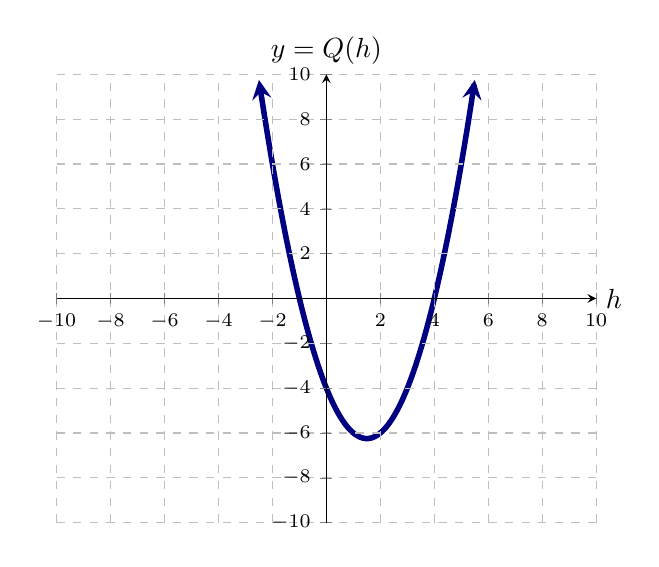
\begin{tikzpicture}
  \begin{axis}[
            domain=-10:10, ymax=10, xmax=10, ymin=-10, xmin=-10,
            axis lines =center, xlabel=$h$, ylabel={$y=Q(h)$}, grid = major, grid style={dashed},
            ytick={-10,-8,-6,-4,-2,2,4,6,8,10},
            xtick={-10,-8,-6,-4,-2,2,4,6,8,10},
            yticklabels={$-10$,$-8$,$-6$,$-4$,$-2$,$2$,$4$,$6$,$8$,$10$}, 
            xticklabels={$-10$,$-8$,$-6$,$-4$,$-2$,$2$,$4$,$6$,$8$,$10$},
            ticklabel style={font=\scriptsize},
            every axis y label/.style={at=(current axis.above origin),anchor=south},
            every axis x label/.style={at=(current axis.right of origin),anchor=west},
            axis on top
          ]
          
            
      		\addplot [line width=2, penColor, smooth,samples=200,domain=(-2.5:5.5),<->] {(x+1)*(x-4)};








  \end{axis}
\end{tikzpicture}
\end{image}



From left to right, the range values, or function values, for $Q$ begin very big and positive.  These values decrease to $0$ and continue negative until they reach a value of $-6.25$. Then, they increase to $0$ again and continue to very big and positive values.

Now we will transform these function values with a linear function.


Let $L(t) = -\frac{1}{4} t + 3$ with domain $\mathbb{R}$.


\begin{itemize}
\item $L$ will take a function value from $Q$ and compress it by a factor of $\frac{1}{4}$. Our parabola will be squished vertically a bit. 
\item Then $L$ will negate the values.  This will vertically reflect the parabola over the horizontal axis.
\item Then $L$ will add $3$ to all of the values.  This will shift the parabola up by $3$.
\end{itemize}












\begin{image}
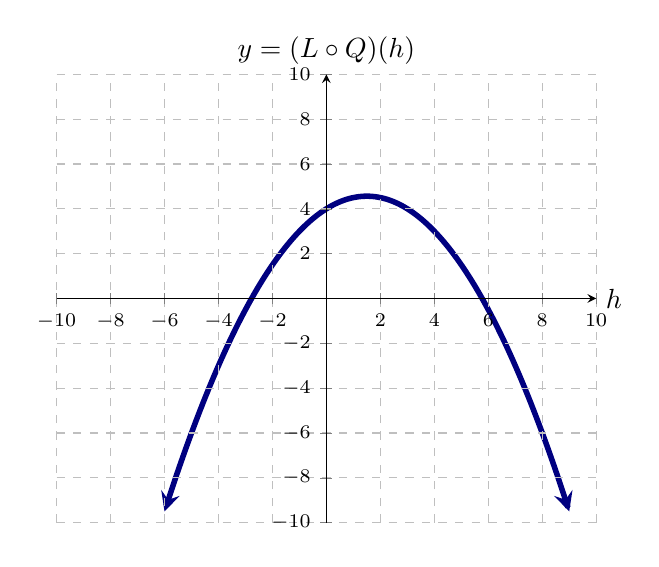
\begin{tikzpicture}
  \begin{axis}[
            domain=-10:10, ymax=10, xmax=10, ymin=-10, xmin=-10,
            axis lines =center, xlabel=$h$, ylabel={$y=(L \circ Q)(h)$}, grid = major, grid style={dashed},
            ytick={-10,-8,-6,-4,-2,2,4,6,8,10},
            xtick={-10,-8,-6,-4,-2,2,4,6,8,10},
            yticklabels={$-10$,$-8$,$-6$,$-4$,$-2$,$2$,$4$,$6$,$8$,$10$}, 
            xticklabels={$-10$,$-8$,$-6$,$-4$,$-2$,$2$,$4$,$6$,$8$,$10$},
            ticklabel style={font=\scriptsize},
            every axis y label/.style={at=(current axis.above origin),anchor=south},
            every axis x label/.style={at=(current axis.right of origin),anchor=west},
            axis on top
          ]
          
            
      		\addplot [line width=2, penColor, smooth,samples=200,domain=(-6:9),<->] {-0.25*(x+1)*(x-4) + 3};








  \end{axis}
\end{tikzpicture}
\end{image}

The vertical measurements have all been processed linearly, which means the shape doesn't change.  It is still a parabola and all of its features are relatively in the same place.



The minimum of $Q$ is $-6.25$ and this occurrs at $1.5$. We are flipping vertically, so the maximum of the composition is still at $1.5$. There were no horizontal transformations.  The maximum is $L(-6.25) = 4.5625$.




The zeros of $L \circ Q$ occur when $L(t) = 0$, which is at $t = 12$.  Therefore, the zeros of $L \circ Q$ occur when $Q(h) = 12$.





$Q(h) = (h+1)(h-4)$



\begin{align*}
Q(h) = (h+1)(h-4)     &  = 12  \\
h^2 - 3h - 4      & = 12   \\
h^2 - 3h - 16 & = 0  \\
\end{align*}

This does not factor easily.  We'll use the quadratic formula.


\[  h = \frac{-(-3) \pm \sqrt{(-3)^2 - 4 \cdot 1 \cdot (-16)}}{2 \cdot 1}  = \frac{3 \pm \sqrt{73}}{2}     \]


We have two zeros: $\frac{3 + \sqrt{73}}{2}  \approx 5.77$ and $\frac{3 - \sqrt{73}}{2} \approx -2.77$, which agrees with our graph.



\begin{claim} Check These are Zeros


\[   Q(h) = (h+1)(h-4)   \]


\[   L(Q(z)) = -\frac{1}{4} (z+1)(z-4) + 3   \]


Let's verify that $\frac{3 + \sqrt{73}}{2}$ is a zero of $L(Q(z))$.



\[   L \left( Q \left( \frac{3 + \sqrt{73}}{2} \right) \right) = -\frac{1}{4} \left( \frac{3 + \sqrt{73}}{2}+1 \right) \left( \frac{3 + \sqrt{73}}{2}-4 \right) + 3    \]



\[  = -\frac{1}{4} \left( \frac{9 + 6 \sqrt{73} + 73}{4} - 3 \cdot \frac{3 + \sqrt{73}}{2} - 4 \right) + 3    \]


\[  = -\frac{1}{4} \left( \frac{82 + 6 \sqrt{73}}{4} - \frac{9 + 3 \sqrt{73}}{2} - 4 \right) + 3    \]


\[  = -\frac{1}{4} \left( \frac{82 + 6 \sqrt{73}}{4} - \frac{18 + 6 \sqrt{73}}{4} - 4 \right) + 3    \]


\[  = -\frac{1}{4} \left( \answer{\frac{48}{4}} \right) + 3    \]


\[  = -3 + 3   = 0 \]


\end{claim}














\begin{claim} Check These are Zeros


\[   Q(h) = (h+1)(h-4)   \]


\[   L(Q(z)) = -\frac{1}{4} (z+1)(z-4) + 3   \]


Let's verify that $\frac{3 - \sqrt{73}}{2}$ is a zero of $L(Q(z))$.



\[   L \left( Q \left( \frac{3 - \sqrt{73}}{2} \right) \right) = -\frac{1}{4} \left( \frac{3 - \sqrt{73}}{2}+1 \right) \left( \frac{3 - \sqrt{73}}{2}-4 \right) + 3    \]



\[  = -\frac{1}{4} \left( \frac{\answer{9 - 6 \sqrt{73} + 73}}{4} - 3 \cdot \frac{3 - \sqrt{73}}{2} - 4 \right) + 3    \]


\[  = -\frac{1}{4} \left( \frac{82 - 6 \sqrt{73}}{4} - \frac{9 - 3 \sqrt{73}}{2} - 4 \right) + 3    \]


\[  = -\frac{1}{4} \left( \frac{82 - 6 \sqrt{73}}{4} - \frac{18 - \answer{6 \sqrt{73}}}{4} - 4 \right) + 3    \]


\[  = -\frac{1}{4} \left( \frac{48}{4} \right) + 3    \]


\[  = -3 + 3   = 0 \]


\end{claim}















\begin{center}
\textbf{\textcolor{green!50!black}{ooooo-=-=-=-ooOoo-=-=-=-ooooo}} \\

more examples can be found by following this link\\ \link[More Examples of Transforming the Outside]{https://ximera.osu.edu/csccmathematics/precalculus1/precalculus1/transformationsOutside/examples/exampleList}

\end{center}




\end{document}
